% Required packages: booktabs, graphicx, subcaption, multirow, xcolor
\section{Experiments}
\label{sec:experiments}

We evaluate Corruption Bias Calibration (CBC) from three complementary perspectives.
First, we verify whether CBC itself improves the zero-shot prediction of CLIP under corruptions, since this is the source of the pseudo labels used by CLIP-based test-time adaptation (TTA) methods.
Second, we stress-test the core assumption of CBC under mixed corruptions, mixed severity levels, class imbalance, and different batch sizes.
Third, we study whether the calibrated pseudo labels are useful when CBC is inserted into existing TTA pipelines.
All reported accuracies are top-1 accuracies in percentage points.

\subsection{Experimental Setup}
\label{subsec:experimental_setup}

\noindent\textbf{Datasets and evaluation protocol.}
We use CIFAR-10 and CIFAR-10-C as the main benchmarks.
CIFAR-10-C contains 15 corruption types applied to CIFAR-10 images with five standard severity levels.
Unless otherwise stated, corrupted-image experiments are conducted at severity level 5.
For corruption-wise evaluation, each corruption type is evaluated independently and the final score is the macro average over the 15 corruptions.
For corruption-mixed evaluation, all severity-5 corrupted images are merged into a single evaluation stream.
For severity-mixed evaluation, all corruptions from severity levels 1 to 5 are merged.
Labels are used only for evaluation.

\noindent\textbf{Model and prompt.}
All zero-shot experiments use the same CLIP visual encoder and the default text template,
\emph{``a photo of a \{\}''}.
CBC is applied on top of the CLIP logits and does not update the image encoder, text encoder, or text prototypes.
The default online batch size is 128 unless a batch-size sweep is explicitly performed.

\noindent\textbf{Baselines.}
For online zero-shot comparison, we compare CLIP, CLIP+CBC, CALIP, WaffleCLIP, and CuPL.
These methods operate without assuming access to the full test set before prediction.
For the offline/transductive setting, we additionally compare against InMaP and Frolic, as well as simple logit-space offline controls.
For TTA experiments, we evaluate nine CLIP-based TTA methods: CLIPArTT, UniEnt, STAMP, TDA, AdaContrast, WATT, WATT-OTSU, WATT-UniEnt, and ETTA.
When CBC is combined with TTA, CBC is used only to calibrate the logits that produce pseudo labels; the TTA method itself remains responsible for all model, cache, or adaptation updates.

\subsection{CLIP Zero-Shot Performance under Corruption}
\label{subsec:zero_shot_corruption}

Before applying CBC to TTA, we first ask whether CBC improves the underlying zero-shot predictions of CLIP.
This is important because CLIP-based TTA methods typically use zero-shot predictions, either directly or indirectly, as pseudo labels.
If the pseudo labels are biased by corruption-induced logit shifts, subsequent adaptation can be guided in the wrong direction.
Table~\ref{tab:main_zero_shot} summarizes the main zero-shot results.
On CIFAR-10-C severity 5, CBC improves CLIP from 60.19\% to 66.73\% when each corruption is evaluated independently, giving a gain of 6.53 points.
This gain is larger than those of the online zero-shot enhancement baselines in our comparison.
The same trend remains under the more difficult corruption-mixed stream, where CBC improves CLIP by 4.54 points.

\begin{table*}[t]
\centering
\caption{Main zero-shot results on CIFAR-10 and CIFAR-10-C. ``S5 avg.'' reports the macro average over the 15 severity-5 corruption-wise evaluations. ``S5 mixed'' merges all severity-5 corruptions into a single stream. ``S1--S5 mixed'' merges all severity levels from 1 to 5. CBC consistently improves CLIP and shows the strongest online zero-shot improvement among the compared methods.}
\label{tab:main_zero_shot}
\small
\setlength{\tabcolsep}{5pt}
\begin{tabular}{lccccc}
\toprule
\textbf{Setting} & \textbf{CLIP} & \textbf{CLIP+CBC} & \textbf{CALIP} & \textbf{WaffleCLIP} & \textbf{CuPL} \\
\midrule
Clean CIFAR-10 & 89.25 & \textbf{91.16} & 86.89 & 90.77 & 90.33 \\
CIFAR-10-C S5 avg. & 60.19 & \textbf{66.73} & 57.40 & 63.20 & 63.08 \\
CIFAR-10-C S5 mixed & 60.19 & \textbf{64.73} & 57.40 & 63.20 & 63.08 \\
CIFAR-10-C S1--S5 mixed & 72.77 & \textbf{76.46} & 69.87 & 75.54 & 75.05 \\
\bottomrule
\end{tabular}
\end{table*}

Table~\ref{tab:corruption_wise} provides the detailed corruption-wise results.
CBC improves CLIP on all 15 corruption types.
The largest improvements appear on noise-like corruptions such as shot noise, impulse noise, and Gaussian noise, where the original CLIP predictions suffer from strong class-wise logit bias.
This supports our claim that CBC is not merely improving an averaged metric, but is consistently reducing corruption-induced prediction bias across diverse shifts.

\begin{table*}[t]
\centering
\caption{Corruption-wise zero-shot accuracy on CIFAR-10-C severity 5. Each corruption is evaluated independently. CBC improves CLIP for every corruption type and obtains the best macro-average performance among online zero-shot methods.}
\label{tab:corruption_wise}
\scriptsize
\setlength{\tabcolsep}{3.2pt}
\begin{tabular}{lrrrrrr}
\toprule
\textbf{Corruption} & \textbf{CLIP} & \textbf{CLIP+CBC} & \textbf{$\Delta$} & \textbf{CALIP} & \textbf{WaffleCLIP} & \textbf{CuPL} \\
\midrule
Brightness & 83.41 & \textbf{86.70} & +3.29 & 80.57 & 85.72 & 85.92 \\
Contrast & 61.94 & \textbf{66.92} & +4.98 & 60.72 & 62.02 & 63.23 \\
Defocus blur & 70.05 & \textbf{74.67} & +4.62 & 66.44 & 73.22 & 71.97 \\
Elastic transform & 53.16 & \textbf{60.90} & +7.74 & 49.12 & 56.53 & 56.71 \\
Fog & 68.43 & \textbf{73.02} & +4.59 & 65.30 & 72.29 & 70.60 \\
Frost & 76.62 & 79.29 & +2.67 & 73.14 & \textbf{79.59} & 78.21 \\
Gaussian noise & 37.83 & \textbf{48.40} & +10.57 & 37.09 & 39.47 & 41.98 \\
Glass blur & 42.20 & \textbf{48.05} & +5.85 & 39.53 & 43.62 & 40.76 \\
Impulse noise & 51.72 & \textbf{62.63} & +10.91 & 48.65 & 58.10 & 59.46 \\
JPEG compression & 56.13 & \textbf{62.44} & +6.31 & 53.23 & 62.10 & 60.08 \\
Motion blur & 65.88 & \textbf{72.62} & +6.74 & 62.33 & 70.79 & 70.87 \\
Pixelate & 48.44 & \textbf{57.33} & +8.89 & 45.55 & 49.38 & 49.99 \\
Shot noise & 41.19 & \textbf{52.83} & +11.64 & 39.78 & 44.34 & 46.84 \\
Snow & 73.31 & \textbf{77.71} & +4.40 & 69.95 & 76.09 & 75.02 \\
Zoom blur & 72.55 & \textbf{77.37} & +4.82 & 69.64 & 74.81 & 74.51 \\
\midrule
\textbf{Average} & 60.19 & \textbf{66.73} & \textbf{+6.53} & 57.40 & 63.20 & 63.08 \\
\bottomrule
\end{tabular}
\end{table*}

\subsection{Robustness of CBC}
\label{subsec:robustness}

\noindent\textbf{Mixed corruptions and mixed severities.}
CBC estimates a shared corruption bias from the batch-level logit statistics.
Therefore, we evaluate whether the method remains effective when the test stream is more heterogeneous than a single fixed corruption.
As shown in Table~\ref{tab:main_zero_shot}, CBC remains effective under both corruption-mixed and severity-mixed evaluation.
In the corruption-mixed stream, CBC improves CLIP by 4.54 points.
In the severity-mixed stream, where severity levels 1 to 5 are all included, CBC improves CLIP by 3.69 points and also outperforms the compared online zero-shot baselines.
These results indicate that CBC is not limited to a single corruption distribution, but can still estimate a useful common bias under realistic mixtures of test-time shifts.

\noindent\textbf{Class imbalance.}
CBC assumes that, within a sufficiently representative batch, the average class evidence should not be dominated by one semantic class.
Under this assumption, the class-wise mean logit can be interpreted as a shift-induced bias rather than as a true semantic prior.
However, if a batch is strongly imbalanced, the batch mean itself can be affected by the semantic composition of the batch.
To test this limitation directly, we construct class-imbalance sweeps for every target class and every corruption type.
The imbalance ratio is varied from 0\% to 100\%, where 100\% means that all samples in the evaluated subset belong to one class.
Figure~\ref{fig:class_imbalance} shows that CBC gradually degrades as the imbalance becomes more severe, which is consistent with its underlying assumption.
Interestingly, CBC remains better than CLIP up to 86\% imbalance.
This suggests that although CBC relies on batch statistics, it is robust to a surprisingly high degree of class imbalance and remains practical for many real-world streams.

\begin{figure}[t]
\centering
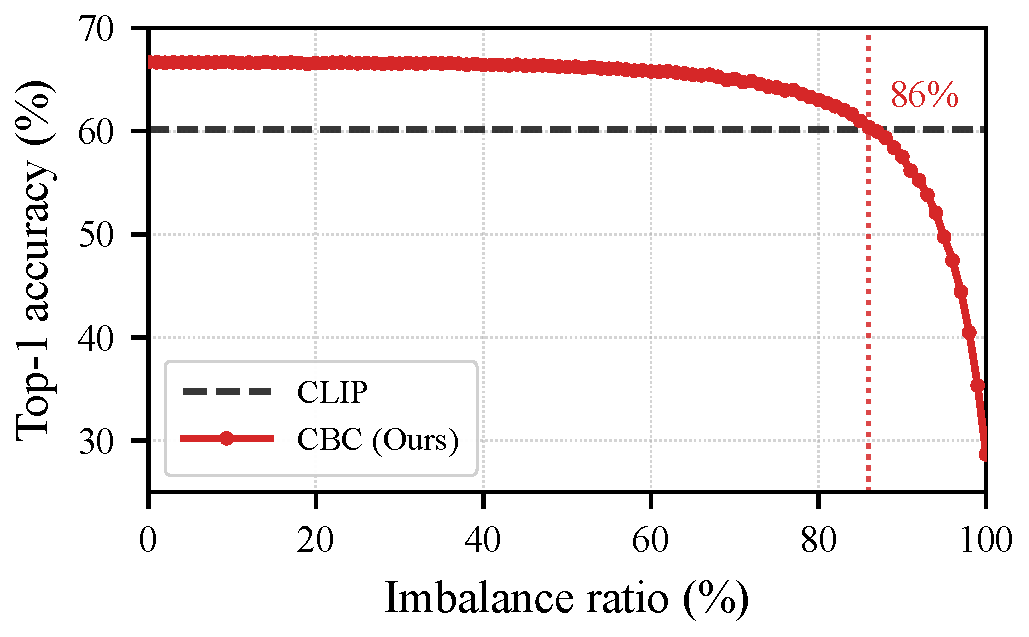
\includegraphics[width=\linewidth]{complete/final_paper_experiments/paper_figures/class_imbalance_sweep_online.pdf}
\caption{Class-imbalance sweep on CIFAR-10-C severity 5. Results are averaged over all 15 corruptions and all 10 target classes. CBC remains above CLIP until 86\% imbalance, after which the semantic prior of the batch begins to dominate the estimated bias.}
\label{fig:class_imbalance}
\end{figure}

\noindent\textbf{Batch size.}
Since CBC uses the batch mean logit as its bias estimate, the batch size directly controls the stability of the estimate.
Figure~\ref{fig:batch_size} shows the batch-size sweep on the corruption-mixed severity-5 stream.
As the batch size increases, the CBC estimate becomes more stable and the performance approaches the large-batch regime.
Very small batches can be unstable because the estimated bias is affected by a small number of samples.
At the same time, CBC does not fundamentally require all samples to be processed in one large batch.
When sufficiently large batches are unavailable, the same principle can be implemented in an online cumulative form by incorporating previously processed samples into the bias estimate.
Thus, CBC can be used either as a batch-wise calibration module or as a streaming calibration module depending on the downstream test-time scenario.

\begin{figure}[t]
\centering
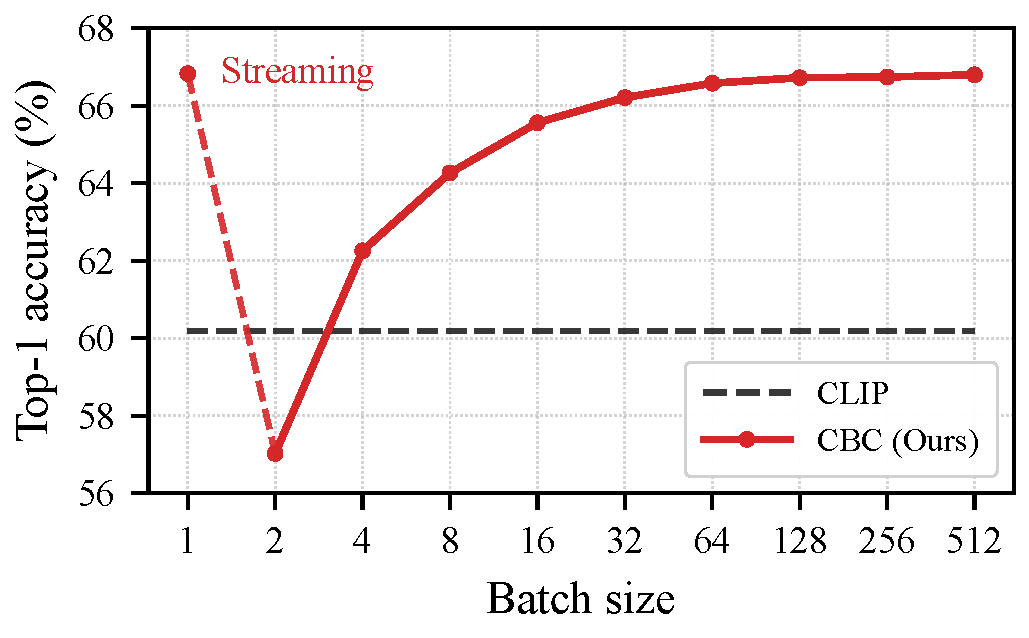
\includegraphics[width=\linewidth]{complete/final_paper_experiments/paper_figures/batch_size_sweep_online.pdf}
\caption{Batch-size sweep on CIFAR-10-C severity 5 with all corruptions mixed. CBC becomes more stable as the batch size grows and consistently exceeds CLIP for moderate-to-large batches.}
\label{fig:batch_size}
\end{figure}

\subsection{CBC in the Offline Setting}
\label{subsec:offline}

Some zero-shot enhancement methods operate in an offline or transductive setting, where the full test set is available before final prediction.
This setting is less restrictive than the online batch-wise setting targeted by CBC, but it is useful for understanding the upper bound of logit-space calibration when global test statistics are available.
We therefore evaluate an offline variant of CBC in the same corruption-wise protocol used in Table~\ref{tab:corruption_wise}: for each severity-5 corruption, CBC computes one global class-wise bias from all 10,000 test logits of that corruption, subtracts it before prediction, and then the final score is averaged over 15 corruptions.
Table~\ref{tab:offline} shows that offline CBC improves CLIP by 6.67 points, reaching 66.86\%.
This is slightly higher than online CBC with batch size 128, as expected from the more stable global bias estimate.
Specialized transductive methods such as InMaP and Frolic achieve higher accuracy, but they rely on full test-set access.
In contrast, the main CBC formulation operates online and can be applied to a batch or stream without requiring the complete test distribution in advance.

\begin{table}[t]
\centering
\caption{Offline/transductive evaluation on CIFAR-10-C severity 5. Results are corruption-wise macro averages. Offline CBC computes one global class-wise bias for each corruption before prediction.}
\label{tab:offline}
\small
\begin{tabular}{lrr}
\toprule
\textbf{Method} & \textbf{Top-1} & \textbf{$\Delta$ vs. CLIP} \\
\midrule
CLIP & 60.19 & 0.00 \\
CBC Offline & 66.86 & +6.67 \\
InMaP & \textbf{69.53} & \textbf{+9.34} \\
Frolic & 68.72 & +8.53 \\
\bottomrule
\end{tabular}
\end{table}

\subsection{CBC on Clean Images}
\label{subsec:clean}

An interesting observation is that CBC also improves zero-shot CLIP on clean CIFAR-10 images.
This is consistent with the mechanism of CBC.
Even for clean images, CLIP zero-shot prediction is not an ideal one-hot alignment between each image feature and its corresponding text prototype.
From the viewpoint of CBC, clean images can still contain a weaker form of common logit bias induced by the mismatch between image features and text prototypes.
By removing this common bias, CBC makes the class evidence more balanced and improves the final prediction.
As shown in Table~\ref{tab:clean}, CBC improves clean CLIP from 89.25\% to 91.16\%, and the offline variant reaches 91.21\%.

\begin{table}[t]
\centering
\caption{Clean-image zero-shot accuracy on CIFAR-10. CBC improves CLIP even without synthetic corruption, suggesting that common logit bias also exists in standard zero-shot prediction.}
\label{tab:clean}
\small
\begin{tabular}{lrr}
\toprule
\textbf{Method} & \textbf{Top-1} & \textbf{$\Delta$ vs. CLIP} \\
\midrule
CLIP & 89.25 & 0.00 \\
CLIP+CBC & 91.16 & +1.91 \\
CBC Offline & \textbf{91.21} & \textbf{+1.94} \\
CALIP & 86.89 & -2.36 \\
WaffleCLIP & 90.77 & +1.52 \\
CuPL & 90.33 & +1.08 \\
\bottomrule
\end{tabular}
\end{table}

\subsection{Qualitative Analysis}
\label{subsec:qualitative}

CBC does not change the shape of the image feature distribution.
Instead, it subtracts a shared class-wise logit bias and effectively shifts the decision evidence toward a better alignment with the text prototypes.
Therefore, CBC is expected to work well when corruption mostly moves the distribution center while preserving the class structure, and to be limited when the corruption heavily distorts the feature distribution itself.
Figure~\ref{fig:corruption_samples} visualizes one clean sample and its 15 corrupted versions.
Figure~\ref{fig:pca_best_worst} compares two selected corruption cases, brightness and glass blur, in a shared feature-space PCA view.
Brightness illustrates a case where the corrupted distribution remains relatively structured and can be better realigned by a common center correction.
By contrast, glass blur provides a visually more distorted case, where the benefit of center correction is expected to depend more strongly on the residual geometry of the shifted feature distribution.
This qualitative contrast motivates the combination of CBC with TTA: CBC corrects the common center bias, while TTA methods can further adapt model- or cache-level representations to recover distorted distribution structure.

\begin{figure}[t]
\centering
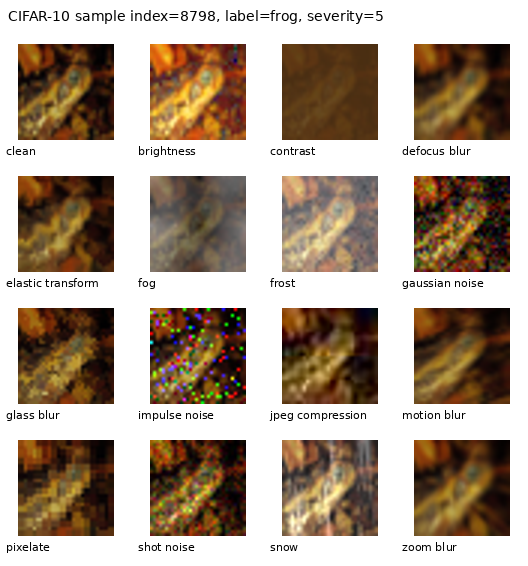
\includegraphics[width=\linewidth]{complete/final_paper_experiments/05_qualitative_analysis/sample_15_corruptions_grid.png}
\caption{Example CIFAR-10 image under the 15 CIFAR-10-C corruption types. The corruptions induce diverse visual shifts, which lead to different degrees of logit bias and feature distribution distortion.}
\label{fig:corruption_samples}
\end{figure}

\begin{figure*}[t]
\centering
\begin{subfigure}{0.48\textwidth}
\centering
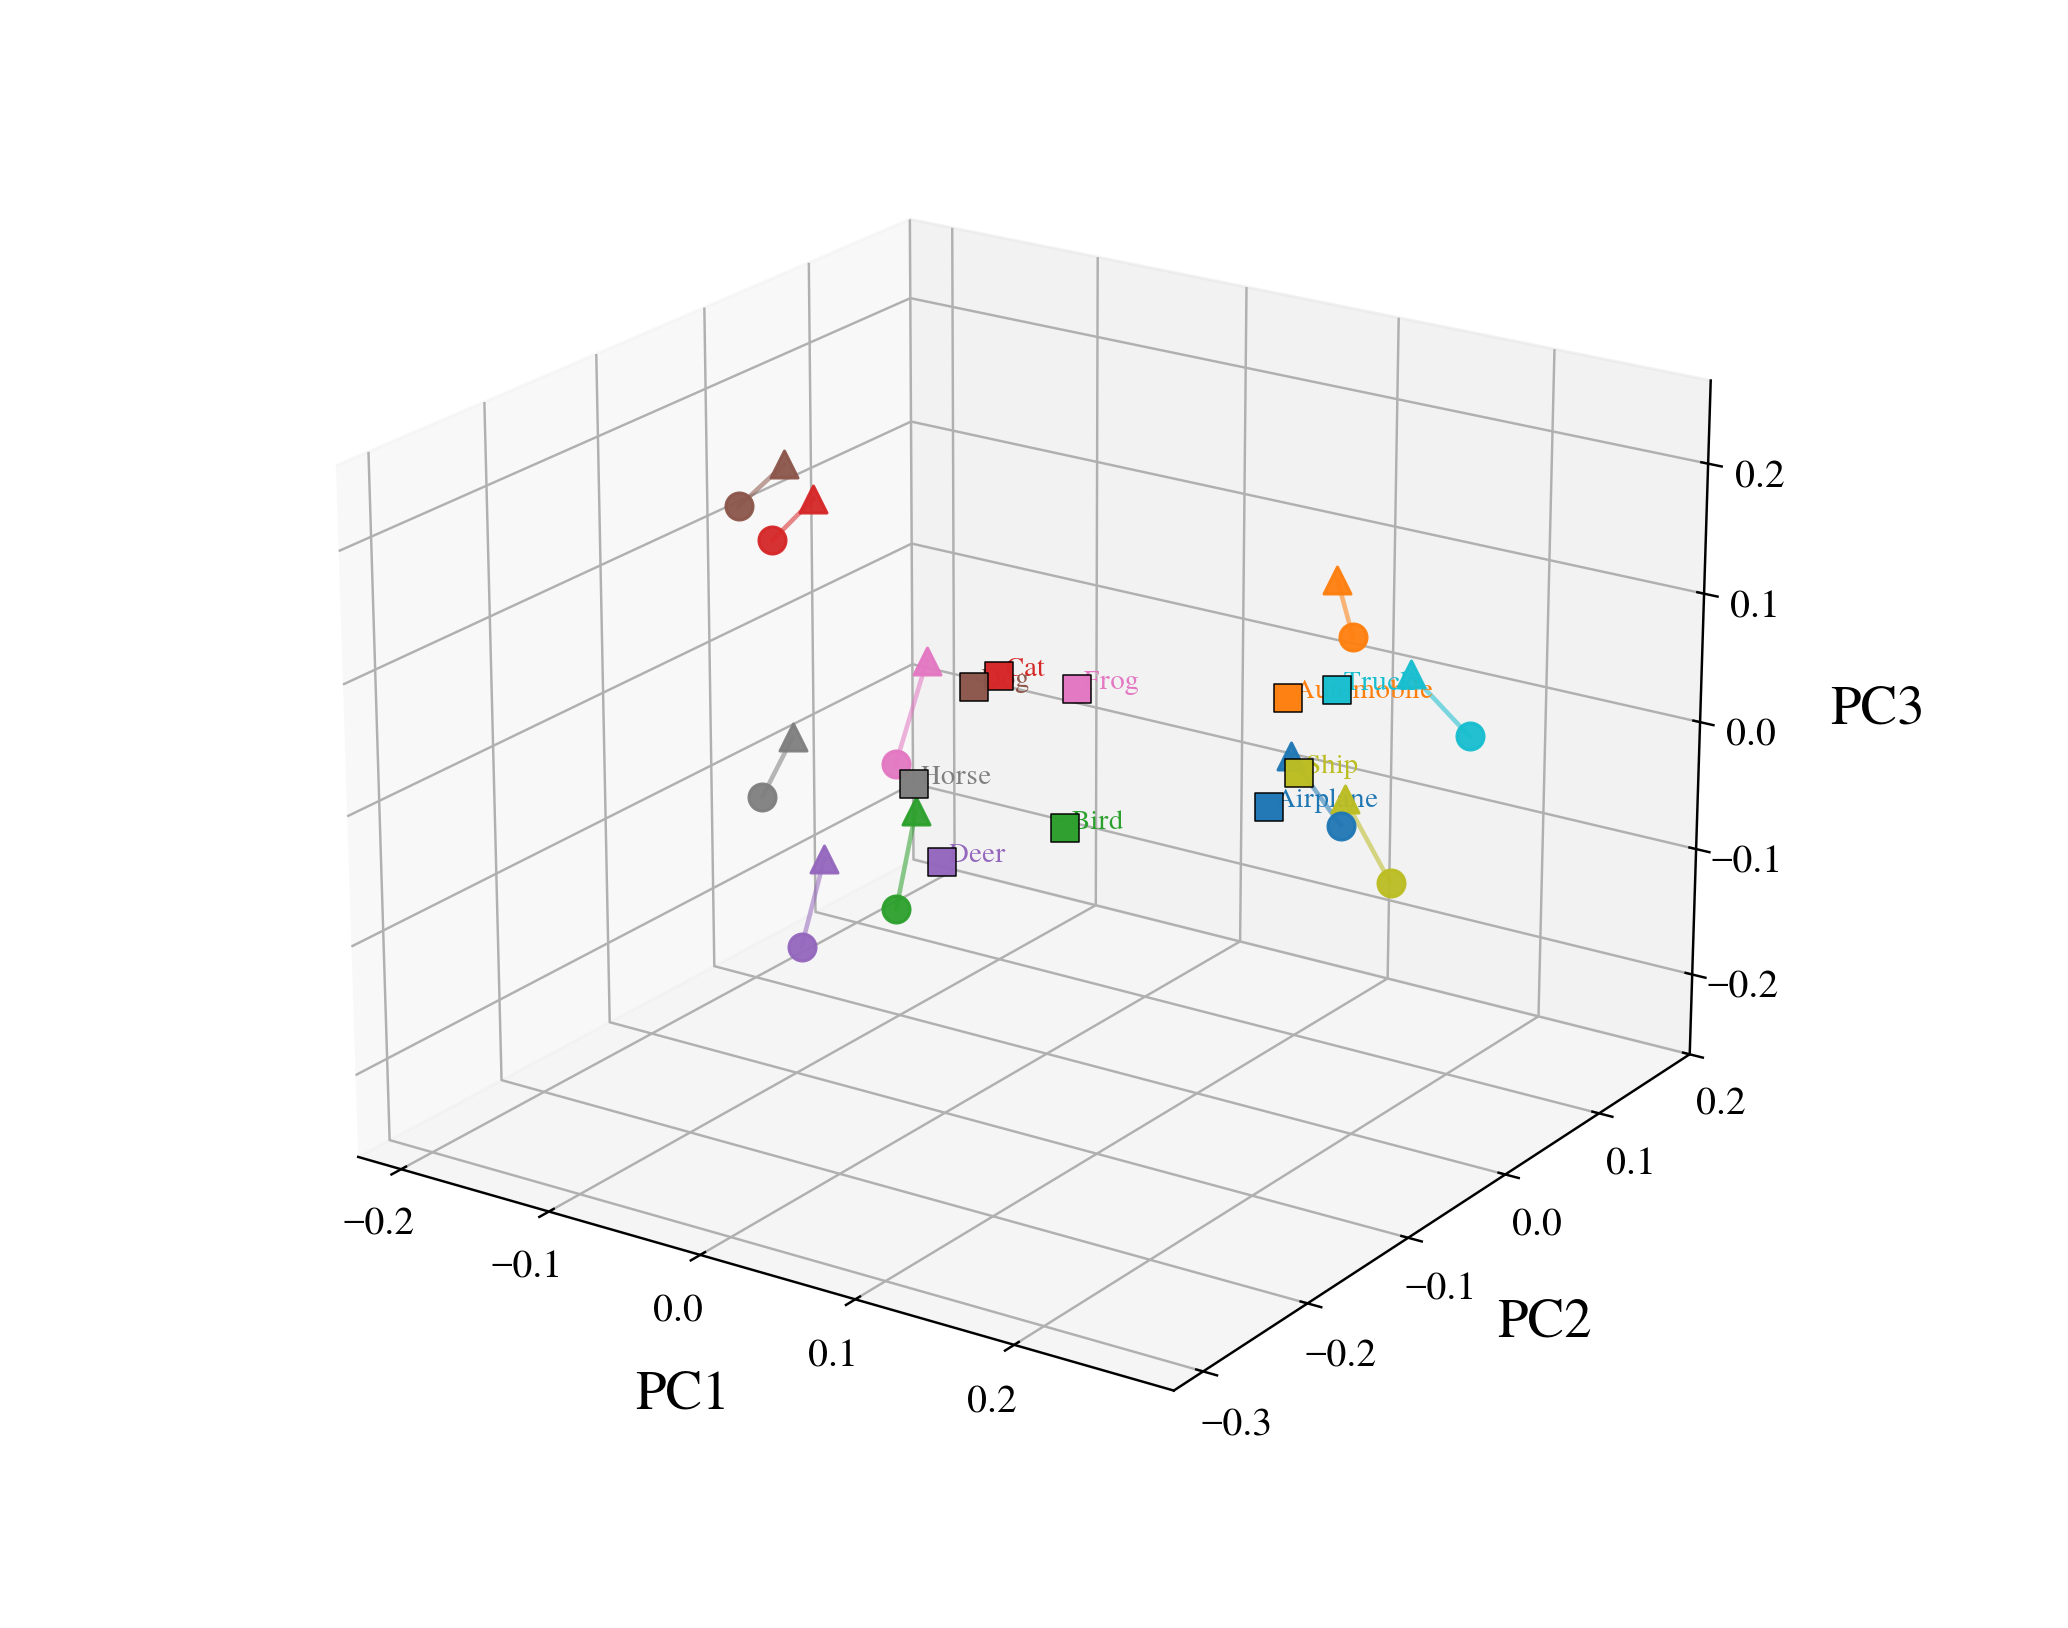
\includegraphics[width=\linewidth]{complete/final_paper_experiments/05_qualitative_analysis/pca_best_brightness/centroids_and_text_pca3d.png}
\caption{Brightness: selected best-case visualization.}
\end{subfigure}
\hfill
\begin{subfigure}{0.48\textwidth}
\centering
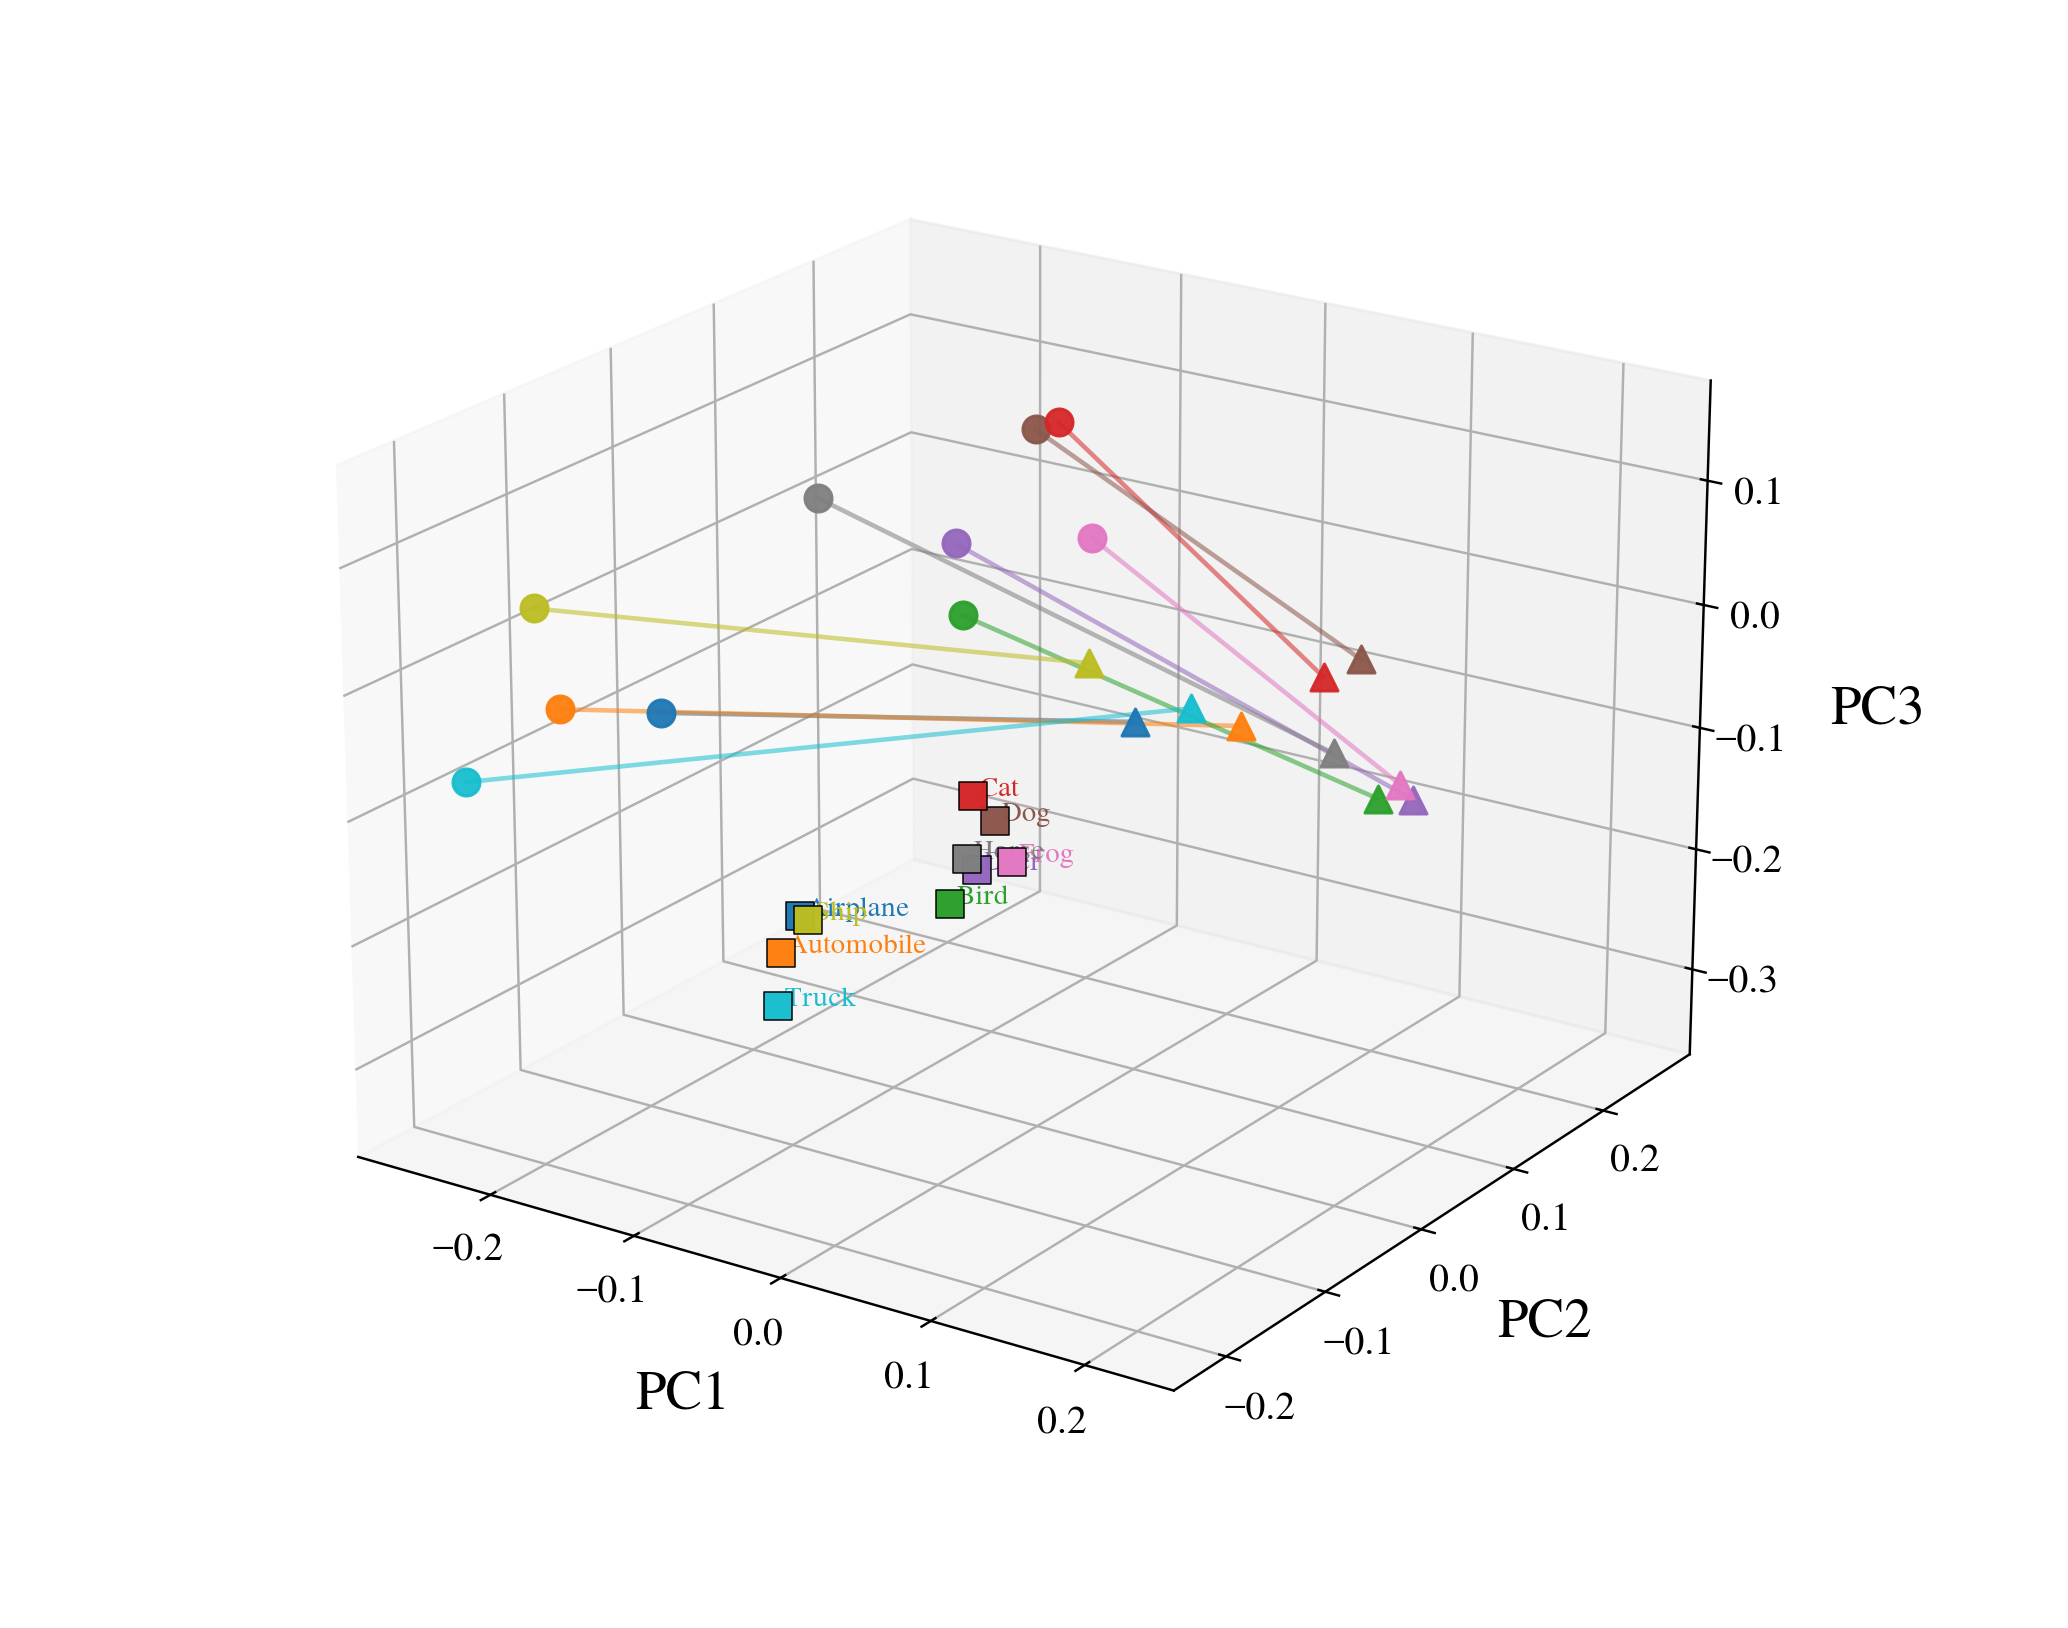
\includegraphics[width=\linewidth]{complete/final_paper_experiments/05_qualitative_analysis/pca_worst_glass_blur/centroids_and_text_pca3d.png}
\caption{Glass blur: selected worst-case visualization.}
\end{subfigure}
\caption{Feature-space PCA analysis for the best and worst corruption types for CBC. CBC is most effective when the corruption mainly shifts the distribution center, while its improvement is more limited when the feature distribution itself is strongly distorted.}
\label{fig:pca_best_worst}
\end{figure*}

\subsection{CBC with CLIP-Based Test-Time Adaptation}
\label{subsec:tta}

Finally, we evaluate CBC as a pseudo-label calibration module for CLIP-based TTA.
CBC and TTA play complementary roles.
CBC does not update the model and does not reshape the feature distribution; it only removes a common logit bias before pseudo-label generation.
TTA methods, on the other hand, can update model parameters, caches, or adaptation states, and therefore can alter the effective feature distribution during test time.
By providing pseudo labels under a better-calibrated decision center, CBC can guide TTA methods toward more reliable adaptation.

Table~\ref{tab:tta} reports corruption-wise macro averages over the 15 CIFAR-10-C severity-5 corruptions.
CBC improves eight out of the nine TTA methods.
Large gains are observed for WATT, WATT-UniEnt, STAMP, and AdaContrast, indicating that pseudo-label calibration can be especially beneficial for methods that are sensitive to initial prediction bias.
UniEnt is the only exception in our results, where CBC reduces the final accuracy.
Overall, these results show that CBC is not only an effective zero-shot correction module, but also a useful plug-in component for improving pseudo-label quality in CLIP-based TTA pipelines.

\begin{table}[t]
\centering
\caption{CBC applied to CLIP-based TTA methods on CIFAR-10-C severity 5. Results are corruption-wise macro averages over 15 independent corruption evaluations. ``Wins'' counts the number of corruptions where TTA+CBC outperforms the corresponding TTA baseline.}
\label{tab:tta}
\small
\setlength{\tabcolsep}{4pt}
\begin{tabular}{lrrrr}
\toprule
\textbf{TTA Method} & \textbf{TTA} & \textbf{TTA+CBC} & \textbf{$\Delta$} & \textbf{Wins} \\
\midrule
CLIPArTT & 68.04 & 71.40 & +3.36 & 15/15 \\
UniEnt & \textbf{79.28} & 75.98 & -3.30 & 0/15 \\
STAMP & 60.17 & 66.70 & +6.53 & 15/15 \\
TDA & 61.84 & 66.46 & +4.61 & 15/15 \\
AdaContrast & 59.68 & 66.05 & +6.37 & 15/15 \\
WATT & 52.75 & 74.93 & \textbf{+22.18} & 13/15 \\
WATT-OTSU & 65.12 & 69.83 & +4.71 & 15/15 \\
WATT-UniEnt & 64.84 & 75.11 & +10.28 & 13/15 \\
ETTA & 62.27 & 66.98 & +4.70 & 15/15 \\
\bottomrule
\end{tabular}
\end{table}

\subsection{Discussion}
\label{subsec:experiment_discussion}

Across the experiments, CBC consistently supports the central hypothesis of this paper: a significant part of CLIP's corruption failure comes from a common class-wise logit bias rather than a complete recognition failure.
When this bias is removed, CLIP zero-shot accuracy improves under corruption, under mixed test streams, and even on clean images.
The class-imbalance and batch-size sweeps also clarify when CBC is expected to work best: the estimated bias should be computed from a sufficiently representative set of samples.
Finally, the TTA experiments show that CBC and adaptation are complementary.
CBC corrects the prediction center used for pseudo-label generation, while TTA can further recover distributional distortions that cannot be solved by a pure logit-bias correction.
